\documentclass[10pt,twocolumn]{article}
\usepackage[margin=0.75in]{geometry}
\usepackage{graphicx,booktabs,amsmath,amssymb,hyperref,xcolor,microtype}
\usepackage[numbers,sort&compress]{natbib}
\hypersetup{colorlinks=true,linkcolor=blue!50!black,citecolor=blue!50!black,urlcolor=blue!50!black}
\title{\textbf{hwsynth: Natural Synthetic Handwriting in 153 Unicode Scripts\\from Writer, Movement and Tool Models}}
\author{pavel9860\\\small\url{https://github.com/pavel9860}}
\date{October 2026}

\begin{document}
\maketitle

\begin{abstract}
Document understanding systems need handwriting in every script they meet, yet learned handwriting generators exist
for a handful of scripts and need large per-script training sets, while rendering handwriting fonts looks
mechanical: every \emph{a} is the same \emph{a}. We present \textsf{hwsynth}, a training-free generator that writes
any text in 153 of the 175 Unicode scripts. Letters are traced from handwriting fonts (Noto where none exists) into
pen paths; a writer model with 44 genes rewrites them; a movement model re-synthesises every stroke as overlapping
lognormal sub-movements and trades shape fidelity against jerk energy by an effort parameter; a tool model with 17
writing instruments deposits ink by nib shape, ink rheology, speed and pressure. Twenty-four handwriting types, grounded
in the discriminating elements of forensic handwriting examination, can each be written in ten situational styles
and with either hand. A quality-diversity search (MAP-Elites) over measured slant and connectedness, scored against real
scanned handwriting with document-disjoint fit and test sets and penalised for baseline instability beyond that of
real handwriting, fills a bank of realistic individuals per type while keeping the types apart in two
writer-identification spaces. On held-out IAM lines the searched bank reaches an embedding Fr\'echet distance of 0.139, closing 71\,\% of the gap between font rendering (0.415) and real handwriting of other forms (0.024); its 24 types are identified with 52\,\% top-1 accuracy (chance 4\,\%).

\end{abstract}

% ---------------------------------------------------------------------------------------------------------------
\section{Introduction}
\label{sec:intro}

Handwriting is everywhere in the documents that machines are asked to read: filled forms, letters, notes,
prescriptions, archives. Training and testing text recognition, layout analysis and document dewarping on
handwriting needs large amounts of it, with exact labels, in every script the system will meet. Collecting and
annotating real handwriting at that scale is slow and, for most of the world's scripts, practically impossible.

Synthetic handwriting is the usual answer, and the field has largely converged on learned generators: recurrent
networks for pen trajectories~\cite{graves2013}, GANs~\cite{fogel2020,kang2020}, transformers~\cite{bhunia2021,pippi2023}
and, most recently, diffusion models~\cite{nikolaidou2023,nikolaidou2024}; see~\cite{diaz2025} for a survey. They
produce convincing samples \emph{for the scripts they were trained on}, almost always Latin and occasionally
Arabic, Chinese or a few Indic scripts, because they need thousands of labelled lines per script and style. For the
other scripts of Unicode, practitioners fall back to rendering handwriting fonts with random affine jitter. The
result is recognisably mechanical: identical glyph instances, perfectly continuous strokes, uniform ink, straight
baselines.

This paper asks whether a generator built from explicit models of \emph{who} writes, \emph{how the hand moves} and
\emph{what tool touches the paper} can close that gap without any trained network. The challenge is that each
model must be faithful enough to remove the mechanical look, and their parameters must be set so that the output
is both realistic and diverse, which no hand-tuning achieves across dozens of interacting parameters.

\paragraph{Contributions.}
\begin{itemize}\setlength\itemsep{1pt}
\item A script-agnostic letter source: centrelines traced from handwriting fonts and Noto fallbacks, drawn per
grapheme cluster or per shaped word, covering 153 Unicode scripts (\S\ref{sec:letters}).
\item A writer model separating \emph{identity} (forensic discriminating elements~\cite{huber1999}) from
\emph{situation}, with 24 handwriting types $\times$ 10 styles $\times$ 2 hands (\S\ref{sec:writer}).
\item A movement model combining lognormal sub-movements~\cite{plamondon1995} with a minimum-jerk~\cite{flash1985}
trade-off controlled by effort, which orders the styles from medical scrawl to calligraphy (\S\ref{sec:motion}).
\item A tool and ink model for 17 instruments after the ink-deposition classes of~\cite{franke2004} (\S\ref{sec:tool}).
\item A leakage-controlled evaluation and a quality-diversity search that scores realism against real handwriting and
separation with image and pen-path writer-identification features~\cite{bulacu2007,lai2019} (\S\ref{sec:evolve}).
\end{itemize}
The code is released under CC BY-NC 4.0 (\S\ref{sec:conclusion}).

% ---------------------------------------------------------------------------------------------------------------
\section{Related Work}
\label{sec:related}

\paragraph{Learned handwriting generation.}
Graves~\cite{graves2013} generated online pen trajectories with an LSTM and mixture density outputs. Haines et
al.~\cite{haines2016} synthesised a specific person's handwriting by assembling and blending their glyphs.
ScrabbleGAN~\cite{fogel2020} and GANwriting~\cite{kang2020} generate offline word images conditioned on content
and style; Handwriting Transformers~\cite{bhunia2021} and VATr~\cite{pippi2023} condition on a few style samples;
latent diffusion models~\cite{nikolaidou2023,nikolaidou2024} currently give the most faithful styles. All require
labelled handwriting in the target script and style, and none covers more than a few scripts.

\paragraph{Perturbation and font based synthesis.}
Before deep generators, synthetic training data came from geometric perturbation of real lines~\cite{varga2003}
and from fonts. Font rendering scales to any script with a font, but repeats glyphs exactly; our letter source
keeps the coverage of fonts and removes the repetition by drawing every glyph as a fresh movement.

\paragraph{Models of handwriting movement.}
The Kinematic Theory~\cite{plamondon1995,plamondon2006} represents a stroke as a sum of lognormal velocity
impulses; its Sigma-Lognormal model reconstructs real trajectories~\cite{ferrer2020} and has been used to design
trajectories~\cite{berio2017}. Minimum-jerk planning~\cite{flash1985} explains the smoothness of point-to-point arm
movements. We use both: lognormal impulses for timing and corner cutting, jerk energy for the effort trade-off.

\paragraph{Individuality of handwriting.}
Forensic examiners compare a set of discriminating elements: allograph design, connections, proportions, slant,
spacing, baseline, commencements and terminations, line quality and natural variation~\cite{huber1999}.
Srihari et al.~\cite{srihari2002} quantified individuality statistically. Automatic writer identification uses
contour-direction and contour-hinge distributions~\cite{schomaker2004,bulacu2007} or path signatures~\cite{lai2019},
grounded in rough path theory~\cite{chen1957,lyons1998}. We use these features to measure and enforce that our types
are distinguishable.

\paragraph{Ink and pencil.}
Franke and Rose~\cite{franke2004} related pen force to ink deposition for solid, viscous and fluid inks; Sousa and
Buchanan~\cite{sousa1999} modelled graphite on paper. Our tool model follows these classes at the cost of a
renderer, not a physical simulation.

\paragraph{Evaluation and search.}
We report Fr\'echet distances~\cite{heusel2017} and k-NN precision and recall~\cite{kynkaanniemi2019} on ImageNet
ResNet18~\cite{he2016} embeddings and on stroke features. The writer bank is filled by MAP-Elites~\cite{mouret2015}, a quality-diversity algorithm that keeps the best
solution in every cell of a behaviour grid, related to novelty search~\cite{lehman2011}.

% ---------------------------------------------------------------------------------------------------------------
\section{Method}
\label{sec:method}

Figure~\ref{fig:pipeline} summarises the pipeline. Text is split into words and drawing units; each unit's glyph
centreline is transformed by the writer, the strokes of a line are moved by the hand, and the tool deposits ink.

\begin{figure}[t]
\centering
\fbox{\parbox{0.94\columnwidth}{\small\centering
\textbf{text} $\rightarrow$ scripts, bidi order, units $\rightarrow$
\textbf{letters} (font centrelines) $\rightarrow$ \textbf{writer} (identity + style genes: shape, layout, joins) $\rightarrow$
\textbf{hand} (lognormal sub-movements, minimum jerk, wrist pivots, tremor) $\rightarrow$
\textbf{tool} (width, density, texture) $\rightarrow$ \textbf{page} (paper, ruling, smudges, word boxes)}}
\caption{The generation pipeline. No stage is learned; the writer bank (\S\ref{sec:evolve}) only selects genes.}
\label{fig:pipeline}
\end{figure}

\subsection{Letters in every script}
\label{sec:letters}
Each character is assigned its Unicode script~\cite{unicode}. Scripts with independent letter forms (Latin,
Cyrillic, Greek, Hebrew, Han, Hangul, \dots) are drawn per grapheme cluster, so every letter gets its own jitter;
all others are shaped by HarfBuzz/Raqm and drawn per word, so joining and conjuncts come from the font. Right-to-left
runs are reversed while digits and Latin runs keep their order. A writer uses its Latin handwriting font for any
script that font covers, otherwise a handwriting font of the script (59 fonts with class labels cursive, print,
brush), otherwise a Noto Sans font (158). A glyph is rasterised at 160\,px, skeletonised, and traced into a graph
whose free spurs are pruned and whose edges continue straight through junctions (smallest turning angle), giving
ordered pen strokes. Glyph size is normalised per script by a reference letter (e.g.\ Han is written at twice the
x-height). Of the 175 scripts in Unicode, 153 have at least one font covering 90\,\% of their core letters.

\subsection{Writers: identity and situation}
\label{sec:writer}
A writer is a vector of 44 genes in $[0,1]$. Twenty-three are \emph{identity} genes following the discriminating
elements of~\cite{huber1999}: size, lateral expansion, ascender and descender length, capital size, slant, letter
and word spacing, line pitch, roundness and angularity (garland, arcade, angular and thread movement), joining,
entry hooks and exit flicks, dot placement and form, pressure, the allograph set (font), the share of letters
written in a second allograph, handedness, all-capital writing, zone flattening and circle-shaped dots. The others are
\emph{situational}: jitter of size, slant, rotation, baseline and spacing (correlated between neighbouring letters,
AR(1) with $\rho=0.6$), speed, effort, decay towards word ends, slant drift, baseline wander, tremor, cross-outs,
retracing and mixed capitals.

A \emph{type} fixes a centre for every identity gene (twenty-four types, Table~\ref{tab:types} in the appendix); an
individual draws each centred gene within $\pm12\,\%$ of its range. A \emph{style} remaps situational genes into
style ranges, keeping each writer's relative position, and shifts a few identity genes (e.g.\ hurried writers join
more and slant further). Left-handed writers (hand gene $>0.9$, about 10\,\%) pull horizontal strokes from right to
left, draw some loops clockwise, write more upright, hold broad nibs steeper and smudge wet ink.

Natural variation comes from four sources: a second allograph for a fixed share of letters, AR(1) letter jitter,
stroke ends that overshoot or stop short, and per-stroke ink-flow drift. Rare events (cross-outs of a misspelt
word, retraced strokes) are drawn from skewed priors.

\subsection{Hand movement}
\label{sec:motion}
Each stroke is reduced to virtual targets (Douglas--Peucker turning points). Segment $j$ becomes a sub-movement
with velocity $\mathbf{D}_j\Lambda(t;t_{0j},\mu_j,\sigma_j)$, where $\Lambda$ is the lognormal impulse response of
the Kinematic Theory~\cite{plamondon1995}; start times are spaced by $2\,o\,e^{\mu-\sigma^2}$, twice the overlap
ratio $o$ times the time of peak speed (isochrony). Fluent writers have small $o$ and cut corners; discrete-stroke
scripts (Han, kana, Hangul, Devanagari) get larger $o$. The integrated path is then the minimiser of
\begin{equation}
  \min_{\mathbf{x}}\;\lambda(\epsilon)\,\lVert\mathbf{x}-\mathbf{p}\rVert^2+\lVert D_3\mathbf{x}\rVert^2,
  \qquad \log_{10}\lambda=-6+6.5\,\epsilon,
\end{equation}
with $D_3$ the third difference (jerk) and end points held: a writer with low effort $\epsilon$ follows the
minimum-jerk path and lets the letter shape go, a writer with high effort keeps the shape and pays in jerk energy.
Effort is a situational gene whose style ranges increase from medical (0--0.12) through hurried, professional,
casual, educated and formal to accurate and calligraphic (0.9--1). The speed of the synthesised movement drives the
tool. Lines follow wrist-pivot arcs that reset at hand shifts every 25--60\,mm, plus slow random baseline wander.

\subsection{Mathematics, chemistry and figures}
\label{sec:math}
Inline \verb|$...$| segments use a small TeX-like syntax: scripts, fractions, roots, Greek letters and symbols, drawn
arrows, \verb|\ce{...}| chemical equations (counts become subscripts, charges superscripts, reaction and equilibrium
arrows) and \verb|\benzene|. They are laid out as boxes of pen strokes: glyph runs come from the writer, rules,
radicals, arrows and rings are drawn as strokes, and the writer's hand then moves over the whole expression like a
word. Figures (circles, ellipses, triangles, rectangles, arrows, stars, ticks, crosses, axes with a curve, underlines)
are planned as freehand paths that do not quite close, overshoot at corners and bow slightly, and are then moved and
inked by the same models.

\subsection{Tools and ink}
\label{sec:tool}
Seventeen tools combine a nib shape (round; broad edge with thick--thin contrast $w+e\lvert\sin(\phi+\alpha)\rvert$
for direction $\phi$ and nib angle $\alpha$; brush with width growing as pressure$^{1.5}$ and tapered ends) with an
ink class~\cite{franke2004}: \emph{solid} (graphite: density follows force, paper grain), \emph{viscous} (ballpoint
paste: density falls with speed, skips on fast strokes, a blob where the pen lands) and \emph{fluid} (gel, rollerball,
fineliner, fountain, markers: near-constant density, pooling at slow points, bleeding halo, darker overlaps).
Pressure combines the writer's push, its variation, extra force on downstrokes, and lift-off ramps. Strokes are drawn
as dense anti-aliased discs at $3\times$ supersampling and combined with tool-specific overlap.

\subsection{Writer bank: quality-diversity search}
\label{sec:evolve}
\paragraph{Real references.} Text lines are cut from 980 scanned handwritten documents, cleaned (no rulings,
staves or bars; contrast; ink share) and kept when most of their five nearest labelled lines are handwriting. The
documents are split into a \emph{fit} set (2\,876 lines) used by the search and a \emph{test} set (1\,181 lines)
used only for metrics; documents whose lines were used to label the handwriting filter are never test documents.

\paragraph{Priors.} Genes a type leaves free are not drawn uniformly: noise genes are drawn as $u^k$
($k=2$--$4$), concentrated near zero, and signed drifts near their centre. Uniform priors gave the median writer
half of the maximum jitter on every noise channel at once, which looks unstable and childish; most adults vary
narrowly to moderately. Fonts with a childish design are reserved for the child type and the uneducated style.

\paragraph{Stability from real handwriting.} Baseline instability is the standard deviation of word ink centres
around their fitted line, in x-heights (estimated from the dense core band of the row profile). On 1\,013 lines
from fit documents it runs from about 0.13 for steady to 0.35 for wavy clean lines; higher values belong to
extraction errors (tables, staves, two lines). Generated and real lines are measured with the same function.

\paragraph{Search.} Each type has a MAP-Elites archive~\cite{mouret2015} over two measured behaviour descriptors:
the slant of near-vertical pen-path segments (7 bins) and pen lifts per letter (5 bins). An individual is rendered on
four search texts, in the casual style and in a random other style. Its quality is
\begin{equation}
  Q=\textit{realism}-4\max(0,\;\textit{instability}-0.15)-[\textit{separation}\le 0],
\end{equation}
where \emph{realism} is the mean of two z-scores (cosine similarity of its line embeddings to their five nearest
fit lines; minus the distance of its stroke features to their five nearest fit lines; both standardised by the same
statistic of fit lines against lines of other documents) and \emph{separation} is the distance to the nearest other
type's centroid minus the distance to its own, in contour-direction/hinge space~\cite{bulacu2007} ($\chi^2$) and in
path-signature space~\cite{lai2019}, each relative to the own distance. New individuals are iso-line variations of
two elites of the same type, kept within the type's range. Finally every elite is re-evaluated with two fresh
seeds and banked when its realism is at least $-0.3$, it is nearer its own type than any other, and its
instability stays below 0.35.

% ---------------------------------------------------------------------------------------------------------------
\section{Experiments}
\label{sec:experiments}

\paragraph{Setup.} Metrics use texts disjoint from the search texts and the held-out test documents. We compare:
plain rendering of a handwriting font (\emph{font}); writers with uniform random genes (\emph{random}); type priors
without search (\emph{prior}); the searched bank (\emph{bank}); and the bank without the pen model, without shape
variation, and without letter joins. Embeddings are ResNet18 (ImageNet)~\cite{he2016}; legibility is the character
error rate of Tesseract~\cite{smith2007} on English lines.

\subsection{Realism and diversity}
Table~\ref{tab:systems} compares the systems on the held-out test documents. Lower Fr\'echet distances (FD) and higher precision and recall mean closer to real handwriting; the first row is the reference level of real handwriting against other real handwriting.
\begin{table*}[t]\centering\small
\begin{tabular}{lrrrrrrrrr}\toprule
system & realism & FD emb. & FD feat. & precision & recall & diversity & writer id & CER & ms/line\\\midrule
real (other documents) & -- & 0.065 & 3.70 & 0.746 & 0.658 & -- & -- & -- & --\\
font rendering & -0.651 & 0.453 & 30.61 & 0.244 & 0.000 & 0.0991 & 0.244 & 0.078 & 5\\
random writers & 0.356 & 0.250 & 20.24 & 0.688 & 0.064 & 0.1189 & 0.588 & 0.524 & 205\\
type priors & 0.331 & 0.248 & 19.94 & 0.669 & 0.023 & 0.1322 & 0.544 & 0.403 & 158\\
evolved bank & 0.383 & 0.245 & 19.13 & 0.688 & 0.015 & 0.1353 & 0.550 & 0.464 & 160\\
bank, no pen model & 0.372 & 0.259 & 19.43 & 0.625 & 0.013 & 0.1325 & 0.475 & 0.455 & 150\\
bank, no shape variation & 0.342 & 0.258 & 18.73 & 0.619 & 0.014 & 0.1376 & 0.544 & 0.430 & 149\\
bank, no joins & 0.364 & 0.249 & 18.93 & 0.613 & 0.020 & 0.1340 & 0.475 & 0.388 & 151\\
\bottomrule\end{tabular}
\caption{Systems against held-out real handwriting (casual style, texts disjoint from the fitness texts).}
\label{tab:systems}\end{table*}

\subsection{Styles and effort}
Table~\ref{tab:styles} lists the bank per style. Movement energy (jerk per unit length of the planned pen path) and turning entropy rise with the effort a style spends on letter shapes, from medical scrawl to calligraphy; legibility follows.
\begin{table}[t]\centering\small\setlength\tabcolsep{3pt}
\begin{tabular}{lrrrrr}\toprule style & realism & FD emb. & energy & entropy & CER\\\midrule
medical & 0.574 & 0.260 & 1.3e-07 & 0.882 & 0.690\\
hurried & 0.528 & 0.254 & 2.7e-07 & 0.926 & 0.568\\
professional & 0.391 & 0.276 & 6.8e-07 & 0.959 & 0.428\\
casual & 0.383 & 0.245 & 1.3e-06 & 0.971 & 0.464\\
unsupported & 0.504 & 0.254 & 1.2e-06 & 0.966 & 0.482\\
educated & 0.384 & 0.269 & 3.3e-06 & 0.996 & 0.507\\
uneducated & 0.452 & 0.284 & 1.5e-06 & 0.976 & 0.285\\
formal & 0.269 & 0.284 & 5.9e-06 & 0.999 & 0.456\\
accurate & 0.290 & 0.322 & 8.2e-06 & 0.997 & 0.209\\
calligraphic & 0.280 & 0.252 & 3.1e-05 & 1.109 & 0.575\\
\bottomrule\end{tabular}
\caption{Evolved bank per style, ordered by effort.}
\label{tab:styles}\end{table}

\subsection{Distinguishable types, individuals and styles}
Table~\ref{tab:dist} reports top-1 nearest-neighbour identification on held-out texts: a type must be recognised from \emph{other} individuals of the type, an individual from its \emph{other} texts, a style from \emph{other} individuals.
\begin{table}[t]\centering\small\setlength\tabcolsep{3pt}
\begin{tabular}{llrrr}\toprule writers & features & type & individual & style\\\midrule
prior & contour hinge & 0.367 & 0.302 & 0.446\\
prior & path signature & 0.375 & 0.504 & 0.532\\
bank & contour hinge & 0.485 & 0.306 & 0.444\\
bank & path signature & 0.519 & 0.486 & 0.569\\
chance & & 0.050 & 0.0125 & 0.200\\
\bottomrule\end{tabular}
\caption{Identification accuracy (20 types, 5 styles).}
\label{tab:dist}\end{table}


\begin{figure*}[t]\centering
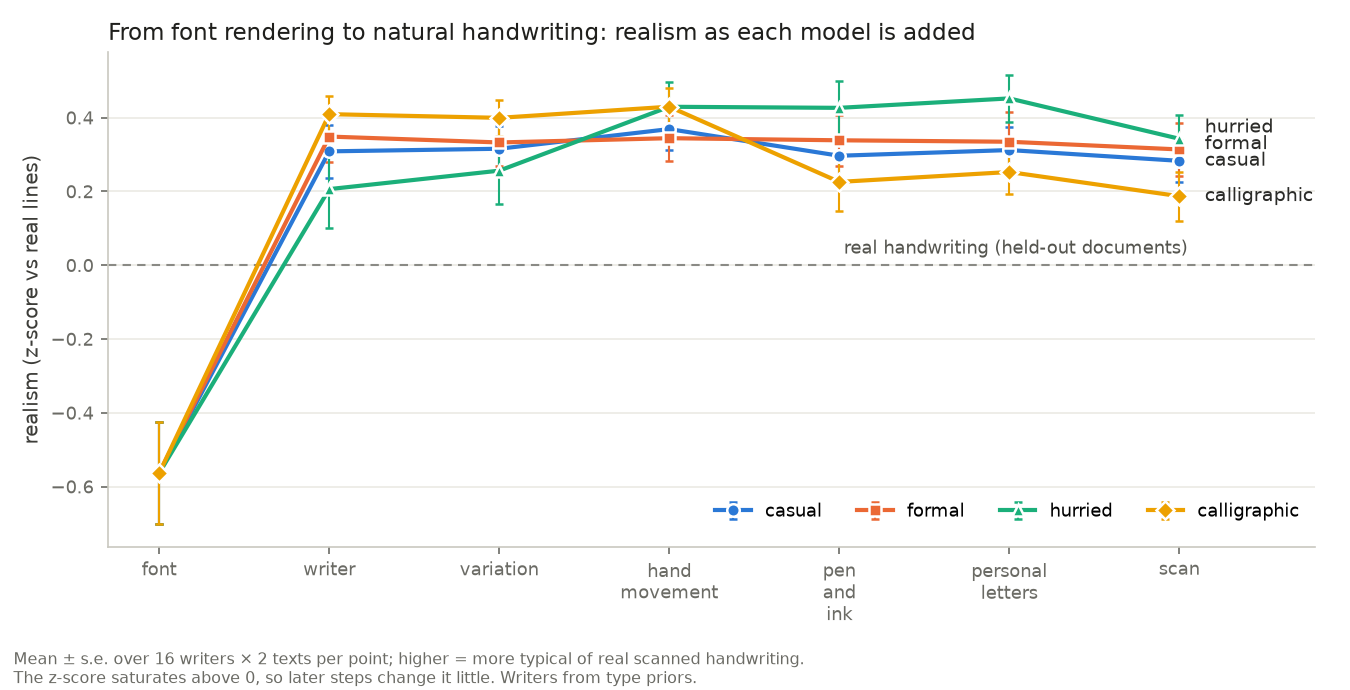
\includegraphics[width=0.62\textwidth]{figs/progression.png}\hfill
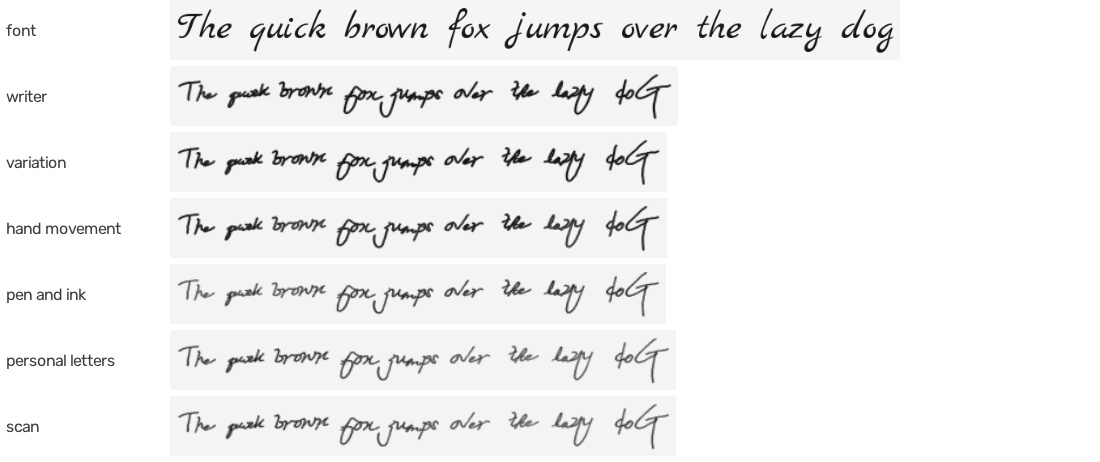
\includegraphics[width=0.36\textwidth]{figs/progression_samples.jpg}
\caption{From font rendering to natural handwriting. Left: realism on held-out real lines as each model is added
(mean $\pm$ s.e., 16 writers $\times$ 2 texts per point). The measure saturates once the output looks like
handwriting, so later stages change it little. Pen and ink lowers the calligraphic style, whose broad-nib contrast
is rare in the mostly ballpoint references. The scan look lowers it slightly too. Right: one writer at each stage.}
\label{fig:progression}
\end{figure*}

\begin{figure*}[t]\centering
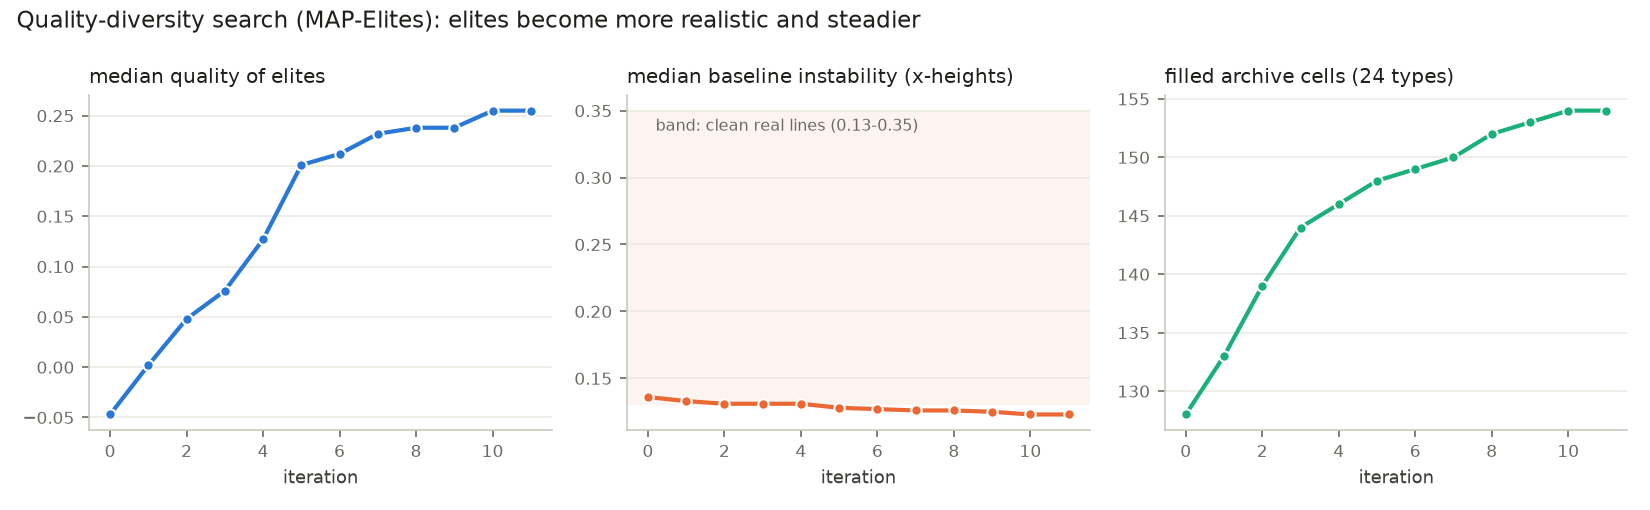
\includegraphics[width=0.95\textwidth]{figs/search.png}
\caption{Quality-diversity search over all 24 types: median elite quality rises from $-0.05$ to $0.26$, median
baseline instability falls inside the range of clean real lines, and the archive fills 154 cells.}
\label{fig:search}
\end{figure*}

\paragraph{Analysis.}
The searched bank closes three quarters of the gap between font rendering and real handwriting in embedding FD
(0.158 against 0.433 for fonts and 0.065 between real documents), with precision 0.69 against 0.34 for fonts. The
scan model is the largest single contributor: without it FD rises to 0.249 and recall falls from 6.4\,\% to
1.6\,\%, although the realism z-score, which saturates and treats scanner noise as atypical, moves the other way
(0.48 against 0.40; Figure~\ref{fig:progression}). Recall remains low: real scans span archives, coloured paper and
damage that the model only partly covers. The search adds realism (0.40 against 0.28 for the type priors) and
precision (0.69 against 0.59) while keeping instability inside the real range (Figure~\ref{fig:search}). Removing
shape variation or letter joins lowers realism and precision; removing the pen model lowers precision and raises FD.
Movement energy rises strictly with the effort of the styles, from medical ($1.7\times10^{-7}$) through hurried,
professional, casual, educated and formal to calligraphic ($3.9\times10^{-5}$), and turning entropy rises with it.
Accurate writing is the most legible style for Tesseract (CER 0.17) and medical writing the least (0.66).
Generation with the scan model takes about 0.3\,s per line on one CPU core.

% ---------------------------------------------------------------------------------------------------------------
\section{Discussion and Limitations}
\label{sec:discussion}
The realism measure is a proxy: ImageNet embeddings and 22 stroke statistics see texture and layout, not the
correctness of letterforms in a particular script, and the reference lines are mostly Latin. No trained writer
identification network was available, so separation uses classical features; the deep writer embeddings of recent
work would be a stronger test. Scripts without a handwriting font inherit Noto's letterforms, which our writer and
movement models make handwritten in execution but not in allograph design. Fitting individuals to real documents by analysis-by-synthesis would ground the bank in real writers.

\section{Conclusion}
\label{sec:conclusion}
Explicit models of the writer, the hand and the tool, set by a leakage-controlled quality-diversity search, produce natural,
diverse handwriting in 153 scripts without any trained generator. Every layer is inspectable: one can ask for a
left-handed elderly writer, in a hurry, with a pencil. Natural extensions are handwriting fonts for the remaining
scripts, page-level phenomena (margins, insertions, marginalia), learned discriminators as realism judges, and
fitting the bank to real writers. Code, examples and this paper: \url{https://github.com/pavel9860}.

{\small\bibliographystyle{plainnat}\bibliography{refs}}

\appendix
\onecolumn
\section{Handwriting types and styles}
\begin{table}[h]\centering\small
\begin{tabular}{lll}\toprule type & fonts & description\\\midrule
school cursive & cursive & taught joined script: loops, right slant, garlands\\
round print & print & rounded upright print, open letters\\
compact print & print & small neat narrow print\\
block capitals & print & everything in capitals, drafting style\\
backhand & any & left-leaning script\\
angular cursive & cursive & sharp, narrow, strongly slanted joined script\\
thready & cursive & fast thread connections, letters dissolve\\
wide garland & cursive & wide open letters, generous spacing\\
narrow tall & any & narrow letters, long ascenders and descenders, tight spacing\\
micro & any & very small writing\\
expansive & any & large writing, big capitals, wide spacing\\
arcade & cursive & rounded tops, slow upright joined script\\
print script & any & print and script mixed\\
elderly & cursive & slow tremulous joined script\\
child & print & large print, uneven baseline, heavy pressure\\
left hooked & any & entry hooks, slight left slant, pressure on downstrokes\\
copperplate & cursive & steep slant, long loops, ornate capitals\\
sloppy fast & cursive & fluent but careless\\
ruled neat & any & very regular, even and aligned\\
artistic & cursive & embellished capitals, exaggerated loops and terminals\\
\midrule style & tools & description\\\midrule
casual & all & everyday notes: as the person writes\\
formal & fountain fine, fountain medium, ballpoint & letters, applications: careful and even\\
accurate & ballpoint, gel, fineliner & forms and labels: separated careful letters\\
calligraphic & broad nib, italic nib, brush pen & broad-nib pen calligraphy: slow, contrasted\\
professional & ballpoint, gel, rollerball & fast, fluent, consistent office notes\\
hurried & ballpoint, ballpoint fine, gel & written in a rush\\
medical & ballpoint, ballpoint fine, gel & prescription scrawl\\
educated & ballpoint, fountain fine, fountain medium & fluent practised writing\\
uneducated & ballpoint, pencil 2b, pencil hb & slow unpractised print, mixed capitals\\
unsupported & ballpoint, gel, pencil hb & on a sheet held in the hand, no support\\
\bottomrule\end{tabular}
\caption{The 20 handwriting types and 10 styles; 17 tools.}
\label{tab:types}\end{table}

\section{Examples}
\begin{figure}[h]\centering
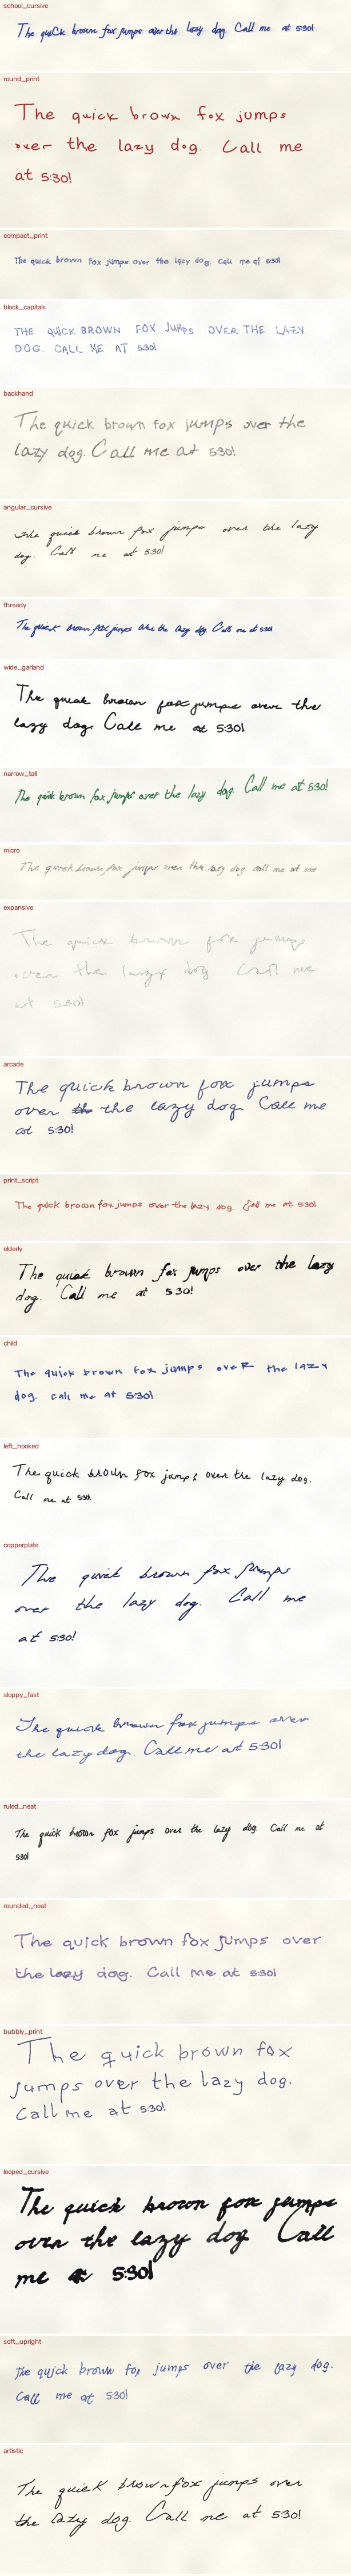
\includegraphics[width=0.95\textwidth,height=0.88\textheight,keepaspectratio]{figs/persons.jpg}
\caption{One individual of each of the 24 types (casual style).}\end{figure}
\clearpage
\begin{figure}[h]\centering
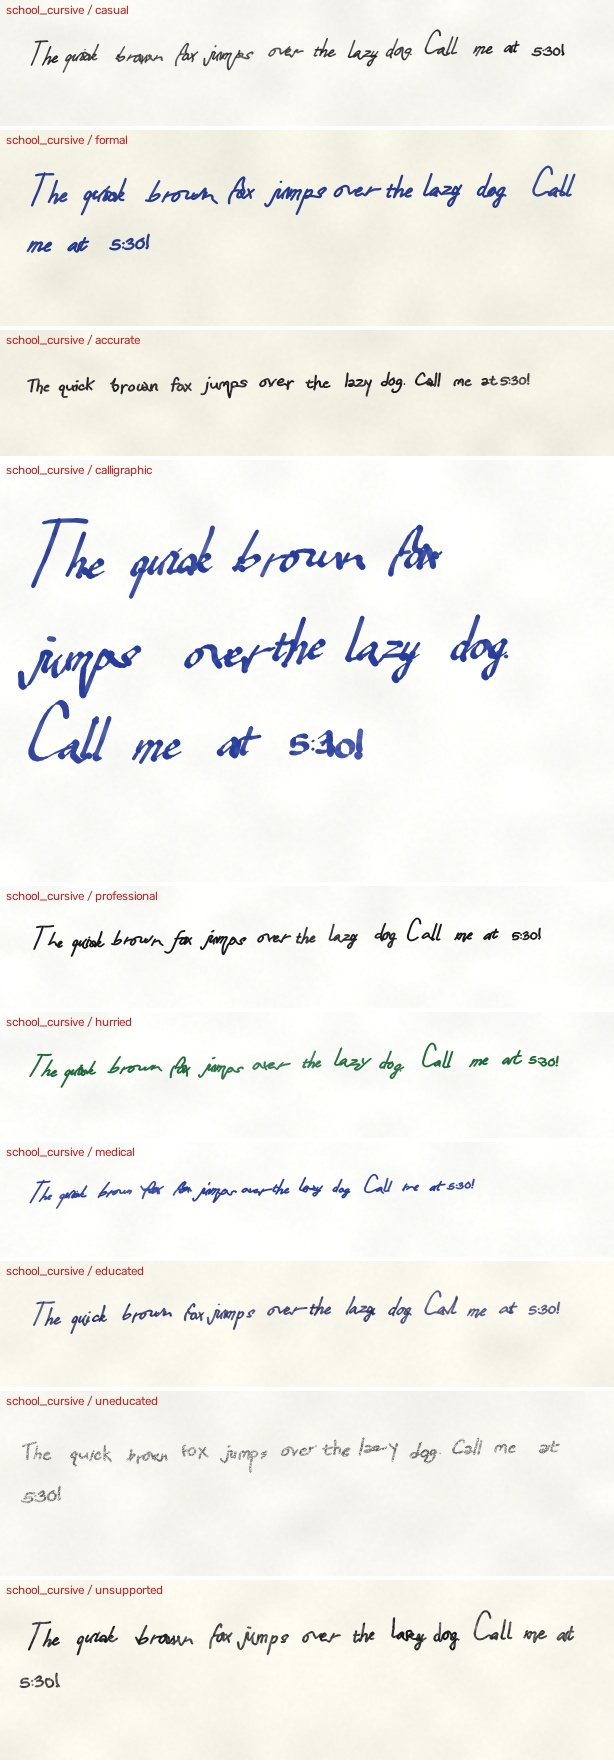
\includegraphics[width=0.95\textwidth,height=0.88\textheight,keepaspectratio]{figs/styles_school_cursive.jpg}
\caption{One school-cursive individual in the 10 styles.}\end{figure}
\clearpage
\begin{figure}[h]\centering
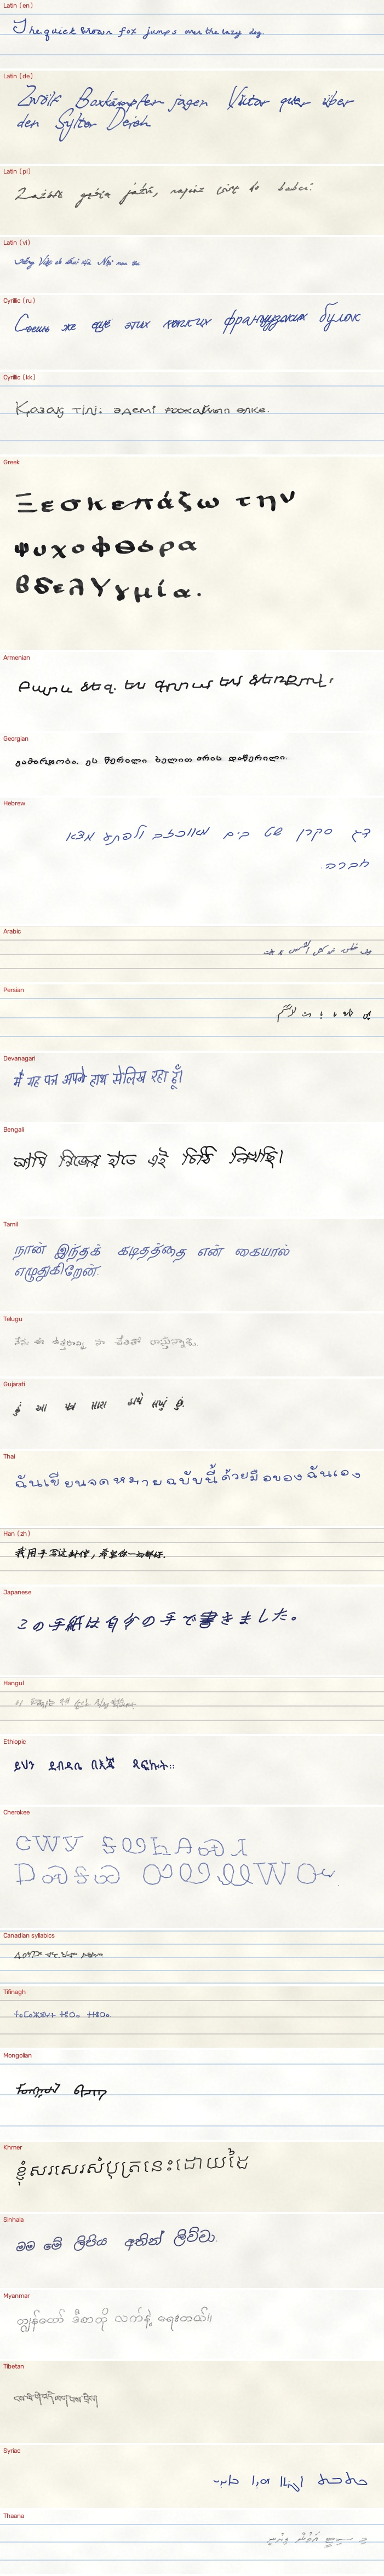
\includegraphics[width=0.95\textwidth,height=0.88\textheight,keepaspectratio]{figs/scripts.jpg}
\caption{Random individuals writing 32 scripts.}\end{figure}
\clearpage
\begin{figure}[h]\centering
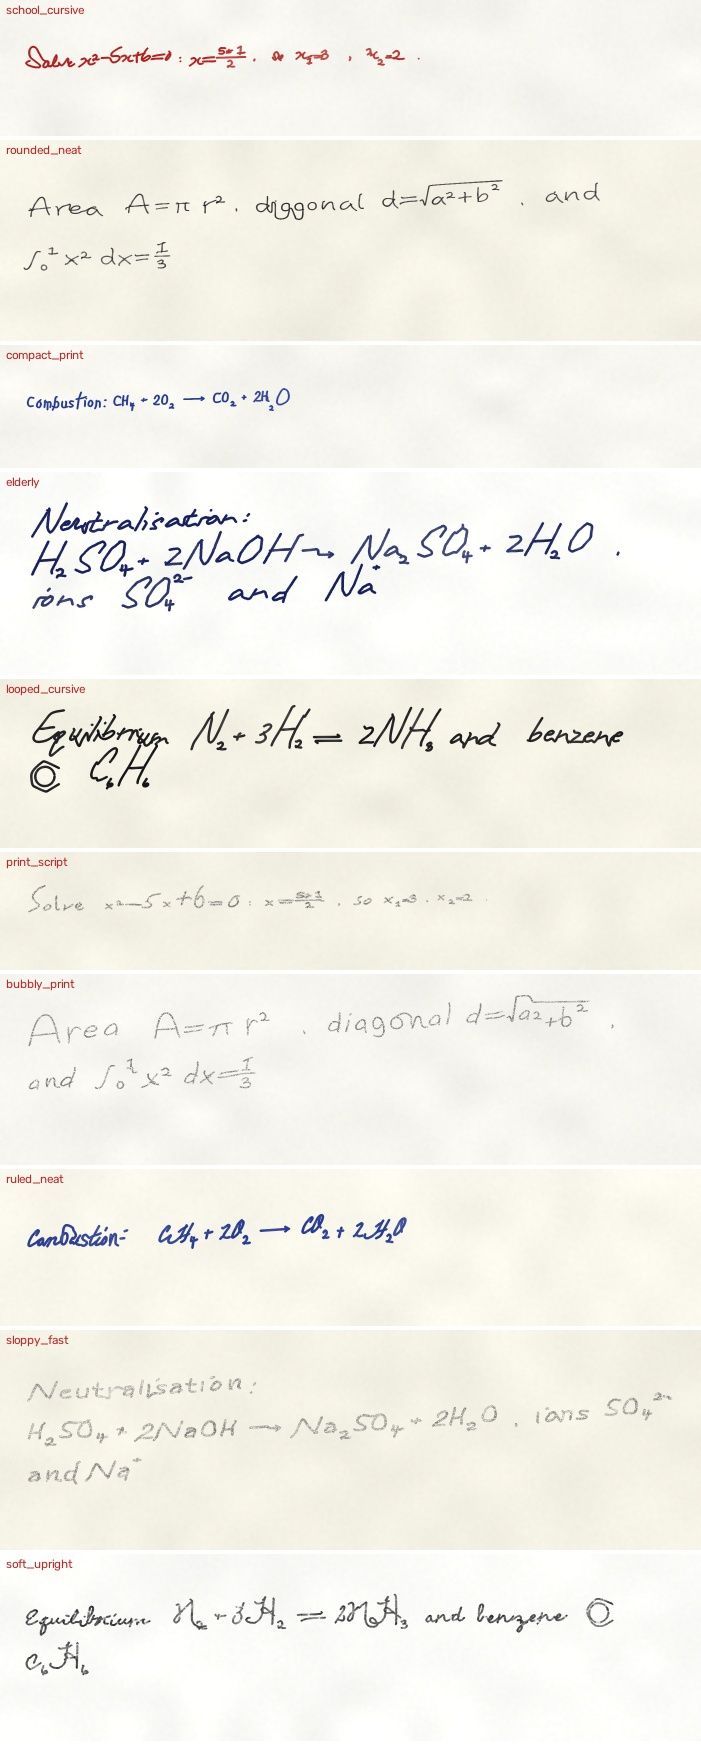
\includegraphics[width=0.95\textwidth,height=0.88\textheight,keepaspectratio]{figs/math_chemistry.jpg}
\caption{Inline mathematics and chemistry.}\end{figure}
\clearpage
\begin{figure}[h]\centering
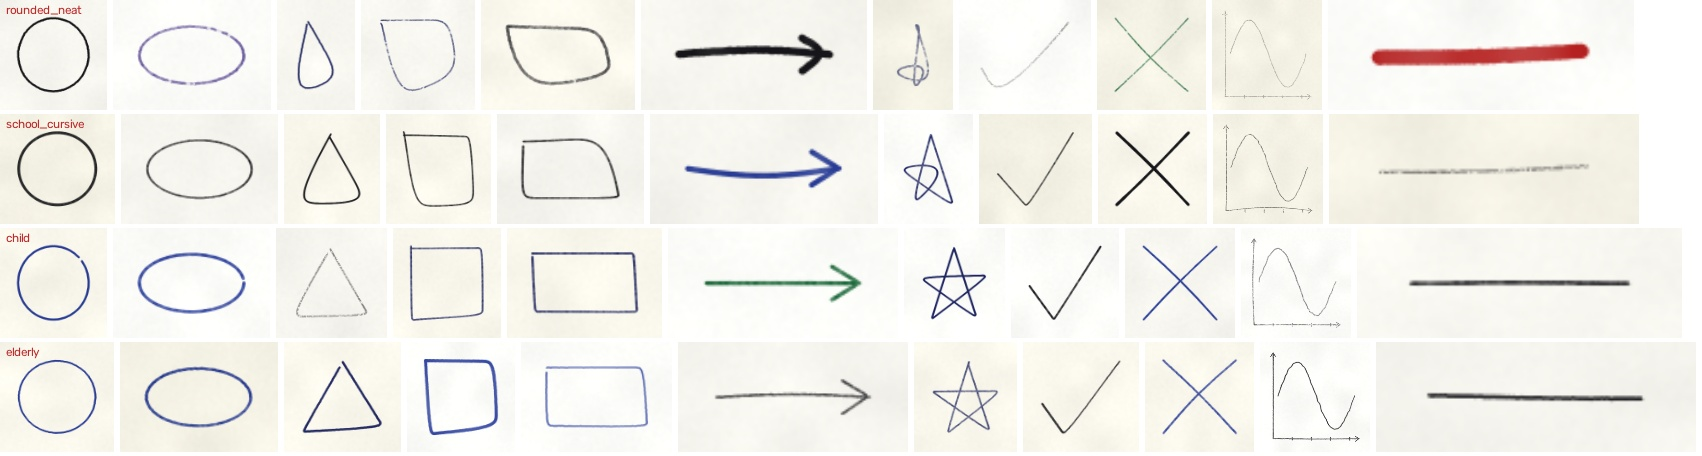
\includegraphics[width=0.95\textwidth,height=0.88\textheight,keepaspectratio]{figs/figures.jpg}
\caption{Hand-drawn figures by four types.}\end{figure}
\clearpage
\begin{figure}[h]\centering
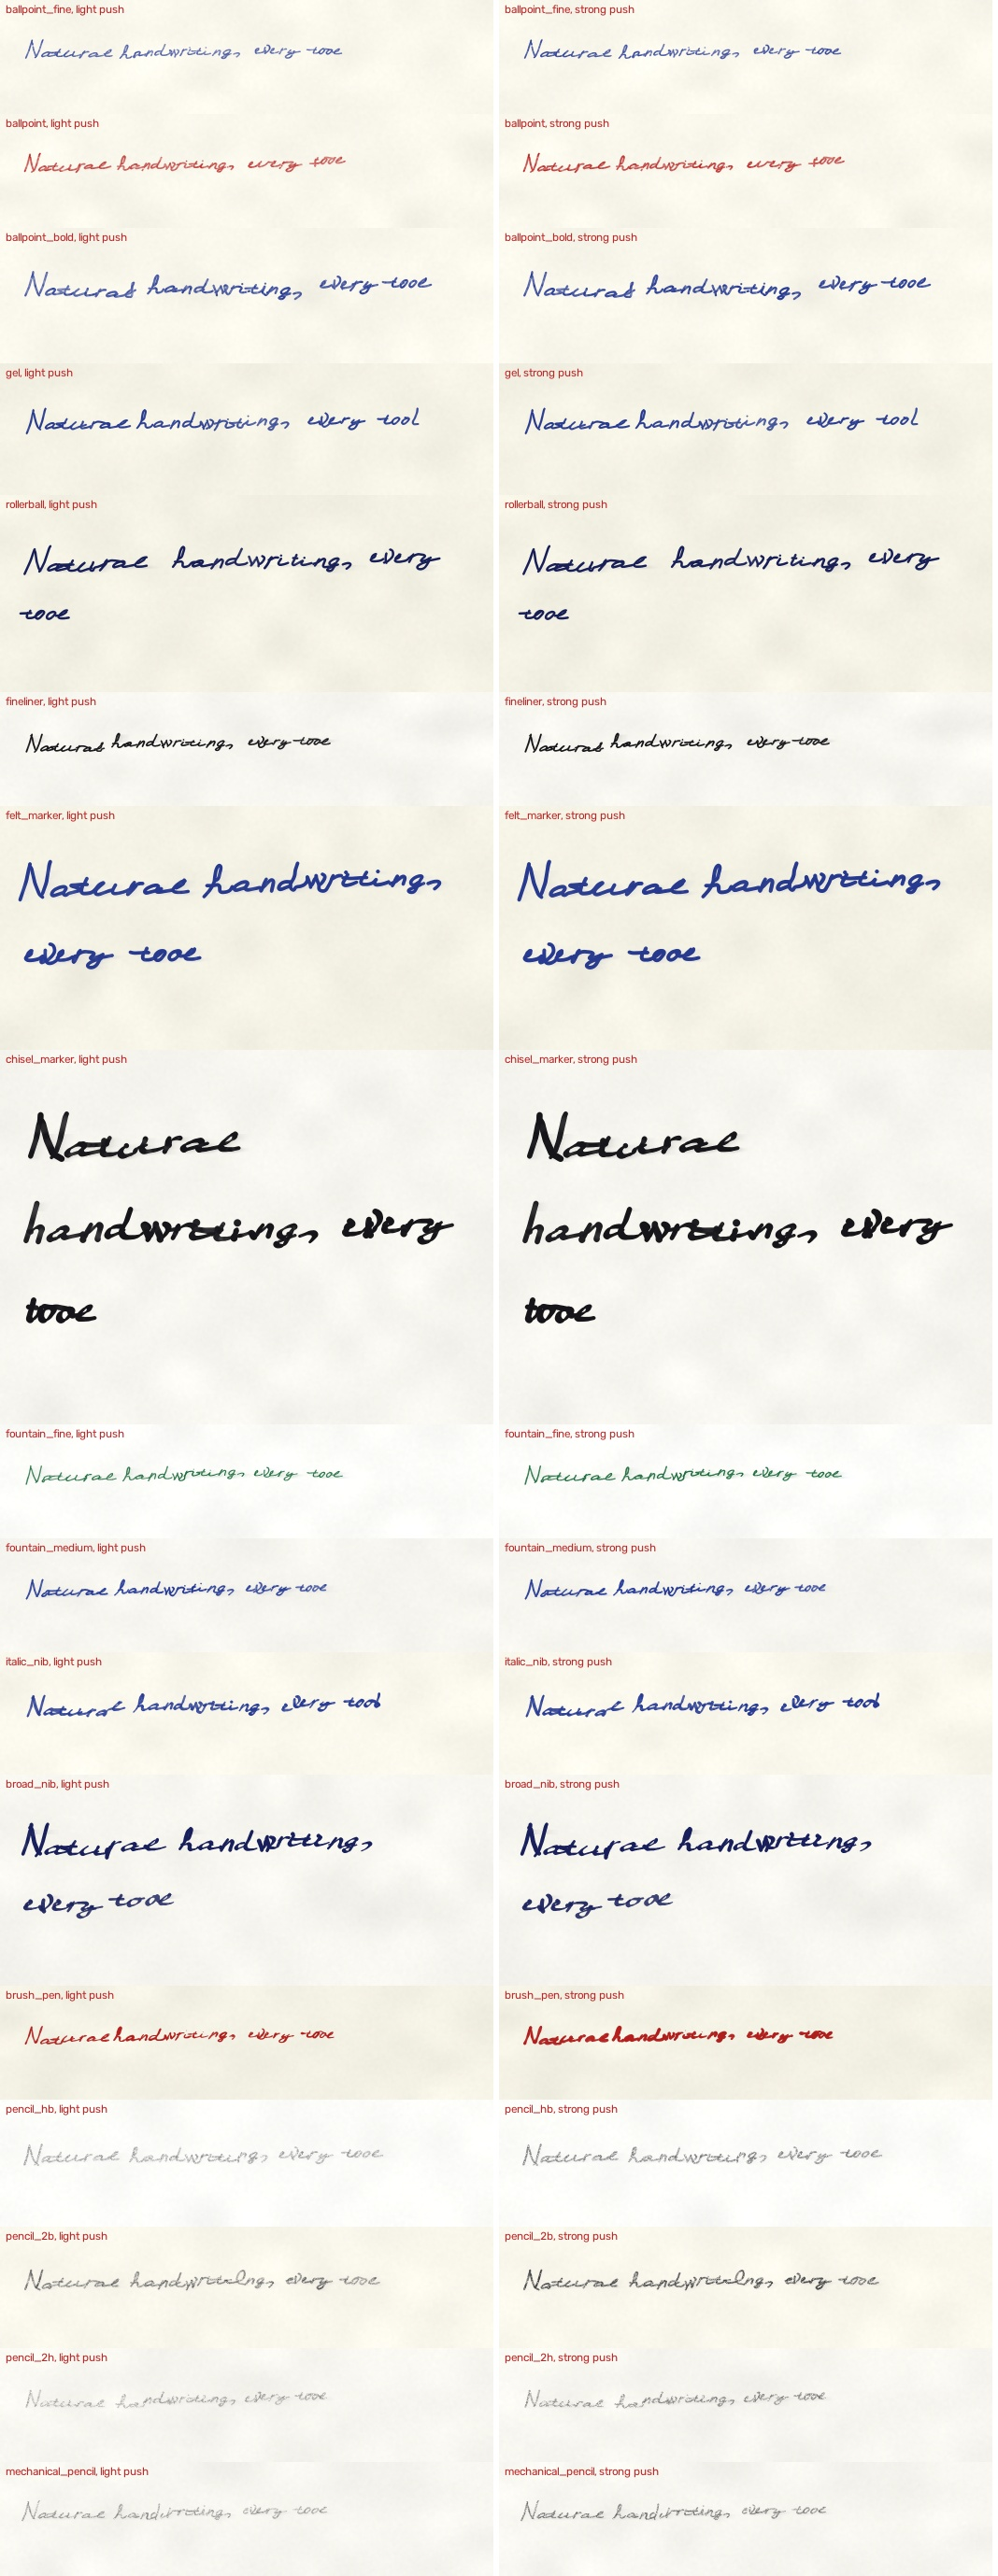
\includegraphics[width=0.95\textwidth,height=0.88\textheight,keepaspectratio]{figs/tools.jpg}
\caption{The 17 tools at light and strong push.}\end{figure}
\clearpage
\begin{figure}[h]\centering
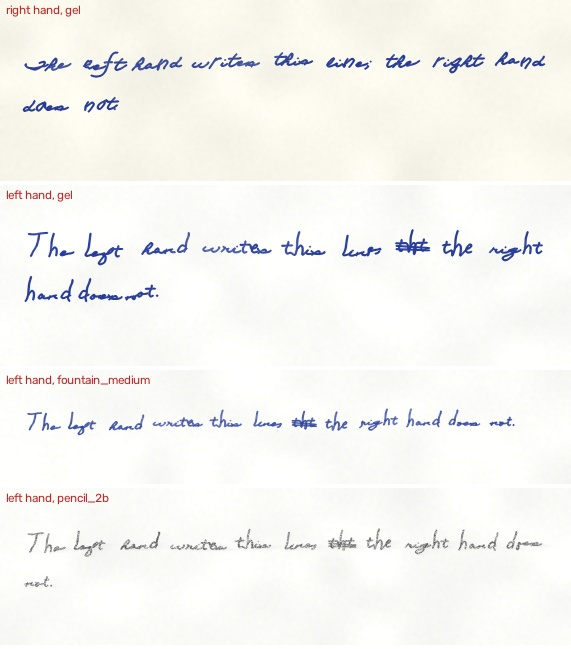
\includegraphics[width=0.95\textwidth,height=0.88\textheight,keepaspectratio]{figs/hands.jpg}
\caption{Right and left hand (gel, fountain pen, pencil): upright slant and smudges.}\end{figure}
\clearpage

\end{document}
